\section{Coleta de estatísticas}
\label{sec:coleta}

A fase de coleta é responsável por solicitar periodicamente estatísticas de fluxo dos \textit{switches} com suporte à OpenFlow e disponibilizar as informações coletadas para a etapa de detecção. Como já discutido na Seção \ref{sec:seguranca}, a análise de fluxo pode ser realizada utilizando dados dos pacotes como endereços \gls{ip} de origem e destino, ou através da análise de \textit{logs} de dispositivos. Tradicionalmente, para análise dos dados dos pacotes, várias técnicas diferentes de monitoramento são utilizadas. Cada técnica de monitoramento requer uma instalação separada de hardware ou configuração de software, tornando isso moroso e com custo alto de implementação. No entanto, OpenFlow  provê as interfaces necessárias para implementar a maioria dos métodos discutidos, sem a necessidade de grandes customizações \cite{Adrichem:2014}.

A definição do intervalo de coleta das entradas de fluxo é de grande importância. Se a coleta é realizada com períodos muito grandes, haverá um atraso na detecção de ataques. Por outro lado, se o intervalo for curto demais, haverá um aumento de tráfego referente às requisições de coleta. Neste trabalho este intervalo foi definido em três segundos com base em resultados obtidos em testes realizados. Este período não produz grande carga na rede e possibilita que várias tentativas de varredura de porta possam ser realizadas, obtendo-se mais fluxos distintos a cada coleta. Também foi adicionado um \textit{timeout} de quinze segundos para os fluxos registrados na tabela de encaminhamento, com isso, a frequência na consulta também permite que as estatísticas de fluxo sejam atualizadas com maior frequência. Apesar desse intervalo possibilitar uma grande quantidade de varreduras antes que as mesmas sejam detectadas, o fato de prover um bloqueio posterior impossibilita que o atacante efetue outros ataques ao término da varredura.

Utilizando as mensagens definidas pelo protocolo OpenFlow e brevemente discutidas na seção \ref{subsec:protocolo-comunicacao}, a coleta de estatísticas é facilitada, passando a ser feita pelo controlador da rede. O controlador realiza, através do protocolo OpenFlow, a coleta de contadores presentes nas tabelas de fluxo dos \textit{switches}. Esses contadores foram definidos com o objetivo de facilitar a criação de mecanismos de \gls{qos} \cite{website:onf} e possuem informações agrupadas por fluxo, por porta, etc. e serão a fonte de informação para este trabalho.

Analisando o que foi discutido na seção \ref{sec:varredura}, técnicas para detecção de varredura de portas podem facilmente ser implementadas utilizando informações do cabeçalho dos pacotes e que também estão presentes nas tabelas de fluxo, como \textit{host} de origem e destino e portas de destino. A fim de se obter estatísticas referentes aos fluxos, OpenFlow fornece alguns métodos para obtenção de informações detalhadas de um fluxo específico, ou de um conjunto de fluxos.

Segundo a especificação OpenFlow \cite{OpenFlowSpec:2014} se o controlador desejar obter estatísticas de um fluxo OpenFlow, ele deve enviar uma mensagem \textit{multipart} (ofp\_multipart\_request) do tipo OFPMP\_FLOW para o \textit{switch}. Mensagens \textit{multipart} são usadas para codificar pedidos ou respostas que podem carregar grande quantidade de informações que nem sempre se encaixam em uma única mensagem OpenFlow, que é limitada a 64KB. O pedido ou resposta é codificada como uma sequência de mensagens de várias partes de determinado tipo em uma mesma conexão, e remontadas pelo receptor. Cada sequência de mensagens \textit{multipart}, carrega apenas uma solicitação ou resposta. Mensagens \textit{multipart} são comumente utilizadas para solicitações de estatísticas ou informações do \textit{switch} \cite{OpenFlowSpec:2014}.

O corpo (\textit{payload}) da mensagem de requisição deve ser preenchido segundo o formato exibido pela Figura \ref{fig:ofp-multipart-request} a seguir:

\begin{figure}[H]
  \centering
  \caption{Estrutura do corpo da mensagem de solicitação de estatísticas}
  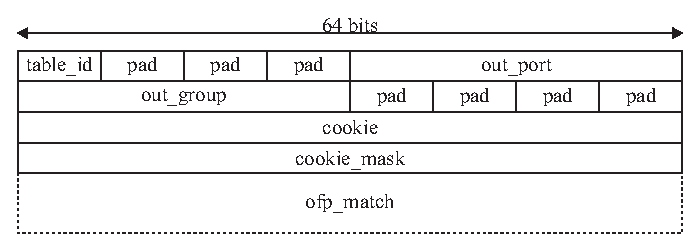
\includegraphics[width=.80\textwidth]{images/ofp-flow-stats-request.eps}
  \label{fig:ofp-multipart-request}
  \fonte{Elaborado pelo autor a partir de\\informações da especificação OpenFlow.}
\end{figure}

O campo \textit{table\_id} deve ser preenchido com o número da tabela onde os fluxos desejados estão armazenados. Se o controlador desejar obter estatísticas de todos os fluxos dessa tabela, apenas essa informação é obrigatória, caso contrário, se o controlador desejar estatísticas de um fluxo específico, devem ser preenchidos os campos de \textit{match}, como endereço de origem e porta destino. Os campos \textit{pad} não necessitam de informação, servem apenas para completar o pacote.

Após enviar a mensagem de requisição, o controlador deve esperar por uma resposta da mensagem pelo \textit{switch}. Se a resposta exceder o limite máximo da mensagem OpenFlow (64KB) o \textit{switch} então, irá enviar uma sequência de múltiplas mensagens com a \textit{flag} OFPMP\_REPLY\_ MORE no cabeçalho da mensagem \textit{multipart} habilitada. 

Se o controlador recebe a mensagem de resposta com esta \textit{flag} habilitada, ele deve armazenar a sequência de mensagens até que a última mensagem da sequência seja recebida. Como o \textit{switch} envia a sequência de mensagens de várias partes com o mesmo ID de transação (xid), o controlador deve mapear todas as partes na sequência e deve ler a mensagem para obter as informações estatísticas.

Quando o \textit{switch} recebe a mensagem OFPMP\_FLOW, ele primeiramente obtém a entrada do fluxo correspondente com base nos campos informados na requisição. Uma vez obtidas as entradas de fluxo correspondentes, o mesmo constrói uma mensagem de resposta (Figura \ref{fig:ofp-flow-stats}) e a envia de volta para o controlador. Esta mensagem pode ser enviada através de um ou mais pacotes, dependendo do tamanho da mesma.

\begin{figure}[H]
  \centering
  \caption{Corpo da resposta à requisição OFPMP\_FLOW.}
  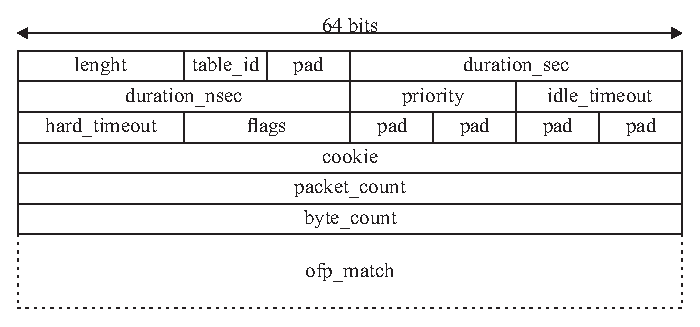
\includegraphics[width=.80\textwidth]{images/ofpmp-flow-stats.eps}
  \label{fig:ofp-flow-stats}
  \fonte{Elaborado pelo autor a partir de informações da especificação OpenFlow.}
\end{figure}

\begin{itemize}
    \item \textit{lenght} indica o tamanho da respectiva entrada de fluxo;
    \item \textit{table\_id} refere-se ao identificador da tabela cujo fluxo foi solicitado;
    \item \textit{duration\_sec} e \textit{duration\_nsec} indicam o tempo decorrido do fluxo desde sua entrada no \textit{pipeline} OpenFlow. A duração total em nano segundos pode ser obtido pelo cálculo $duration\_sec * 10^9 + duration\_nsec$;
    \item \textit{flags} possui informações das \textit{flags} TCP como SYN, ACK e FIN;
    \item \textit{packet\_count} é um contador de medição de pacotes que trafegam com o respectivo \textit{match} desse fluxo;
    \item \textit{byte\_count} indica o número de \textit{bytes} do respectivo fluxo; e
    \item \textit{ofp\_match} é uma lista de zero ou mais propriedades específicas para as regras, como portas de origem e destino, tipo de rede, endereços de origem e destino, etc.
\end{itemize}


O controlador OpenDaylight implementa uma abstração dos pacotes e protocolos utilizados, tornando a tarefa de desenvolver troca de mensagens com os \textit{switches} mais ágil e prática.
A sua estrutura de funcionamento é baseada em uma árvore, o que possibilita o endereçamento de qualquer elemento/sub-árvore que esteja sob o domínio do controlador. Nesta árvore, ilustrada na Figura \ref{fig:arvore-dados}, tem-se o controlador interligado aos \textit{switches}, que por sua vez possuem tabelas e estes, possuem nodos que correspondem às informações de fluxos. Sendo assim, pode-se obter estatísticas de fluxo de um determinado \textit{switch} através da leitura sucessiva de seus nodos. Para obter as estatísticas do primeiro fluxo presente da segunda tabela do primeiro \textit{switch}, deve realizar a leitura do nodo "\textit{Switch} 1", a partir deste nodo pode-se realizar uma leitura de todas as tabelas presentes até que se encontre a "Tabela 2", estando na tabela dois pode-se obter as estatísticas agregadas de fluxo ou de fluxos específicos, que neste exemplo é o "Fluxo 1".

\begin{figure}[H]
  \centering
  \caption{Representação da árvore de dados no OpenDaylight.}
  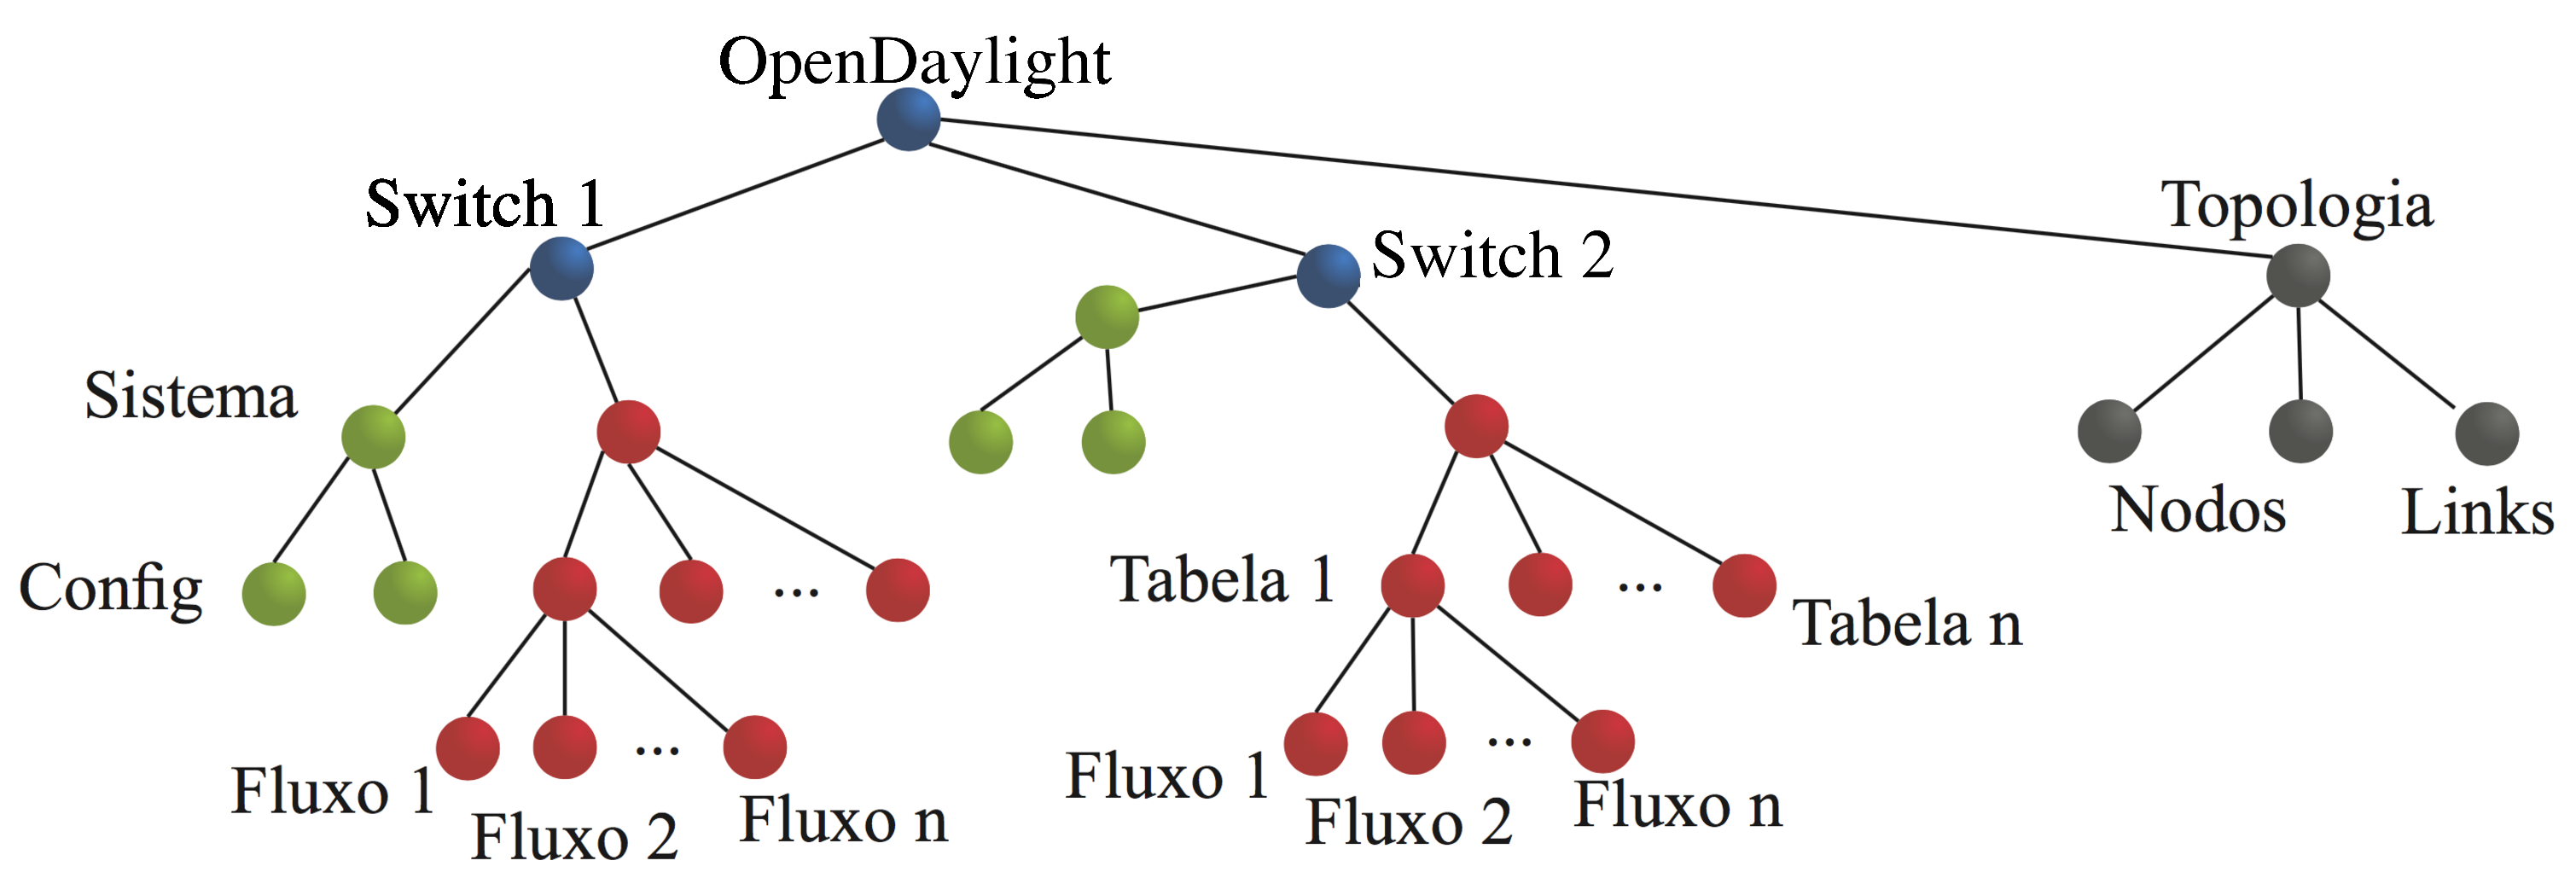
\includegraphics[width=.9\textwidth]{images/arvore.eps}
  \label{fig:arvore-dados}
  \fonte{\centering Elaborado pelo autor com base na especificação OpenDaylight.}
\end{figure}

A configuração dos dispositivos e a coleta de estatísticas de fluxos no OpenDaylight pode ser obtida de forma muito simples através de um \textit{browser} utilizando-se uma \gls{api} chamada \textit{restconf}. Um exemplo de requisição de estatística de fluxo pode ser obtida através do Localizador Uniforme de Recursos (\gls{url}): http://localhost/restconf/config/open- daylight-inventory:nodes/node/openflow:1/table/0/flow/tcipsflow-1

Onde:
\begin{itemize}
    \item http://localhost - é o endereço \gls{web} do controlador;
    \item restconf - é o nome da \gls{api} ao qual está se requisitando a informação;
    \item config - é a base de dados de configuração do OpenDaylight;
    \item opendaylight-inventory:nodes - indica que a partir desse ponto a estrutura é baseada em nodos;
    \item nodo/openflow:1 - indica que o nodo a ser consultado é o chamado openflow:1;
    \item table/0 - indica que a tabela do nodo acima a ser consultada é a de identificação 0; e
    \item flow/tcipsflow-1 - indica que o fluxo de nome "tcipsflow-1" deverá ser consultada na tabela acima.
\end{itemize}

Se o desejado for obter a informação de todos os fluxos da tabela, a informação de fluxo  (\textit{flow}) pode ser omitida da \gls{url}, como por exemplo: http://localhost/restconf/config/openday- light-inventory:nodes/node/openflow:1/table/0. O resultado será um arquivo em formato \gls{json} ou \gls{xml} como exibido na Figura \ref{cod:ofp-flow-stats}.
\begin{figure}[H]
  \centering
  \caption{Corpo da resposta ofp-flow-stats no formato JSON}
\begin{lstlisting}[belowskip=-0.05 \baselineskip]
{ "flow-node-inventory:table": [
    {"id": 0,
      "opendaylight-flow-table-statistics:flow-table-statistics": {
        "packets-looked-up": 37,
        "active-flows": 3,
        "packets-matched": 19 },
      "flow": [
        { "id": "tcipsflow-1",
          "table_id": 0,
          "instructions": {
            "instruction": [
              { "order": 0,
                "apply-actions": {
                  "action": [
                    { "order": 0,
                      "output-action": {
                        "output-node-connector": "CONTROLLER"}}]}}]},
          "priority": 1,
          "opendaylight-flow-statistics:flow-statistics": {
            "duration": { "nanosecond": 583000000, "second": 156 },
            "packet-count": 1, 
            "byte-count": 74 },
          "match": {
            "ethernet-match": { "ethernet-type": { "type": 2048 }},
            "ip-match": { "ip-protocol": 6 }},
          "idle-timeout": 0,
          "hard-timeout": 0 }]}]}
\end{lstlisting}
\fonte{\centering Extraido da interface do OpenDaylight executado pelo autor.}
 \label{cod:ofp-flow-stats}
 \end{figure}
Neste exemplo, cada nodo é representado por um sub-elemento JSON. A tabela possui dados agregados de pacotes transmitidos e fluxos. Cada fluxo por sua vez possui informações de \textit{match} para a verificação do pacote recebido, \textit{instructions}, instruções que devem ser tomadas se os campos em \textit{match} forem satisfeitos, campos de \textit{timeout}, \textit{flags} e estatísticas conforme o especificado pelo protocolo Openflow.
 
Apesar de a coleta ser facilmente realizada através da \gls{api} \textit{restconf}, esta aplicação implementa a coleta diretamente sobre a base de dados do controlador, fazendo uso dos métodos desenvolvidos pela comunidade de desenvolvedores do OpenDaylight. Esta escolha torna-se mais viável considerando-se que esta aplicação foi desenvolvida como uma parte do controlador, tendo portanto, acesso direto à sua base de dados e dispositivos. Na Figura \ref{cod:code-colection} é ilustrada a obtenção de um fluxo diretamente da base de dados OpenDaylight. Neste exemplo cada elemento da árvore deve ser verificado até que o nodo que contém informações de fluxo seja encontrado.

\begin{figure}[H]
  \centering
  \caption{Exemplo para obtenção de estatísticas da base de dados do OpenDaylight}
\begin{lstlisting}[belowskip=-0.05 \baselineskip]
Nodos nodos = obterNodosDaBaseDeDados();
/* Iteracao sobre cada nodo */
for (Iterator<Node> iterator = nodes.getNode().iterator(); 
    iterator.hasNext();) {
  
  Node childNode = iterator.next();
  /* Iteracao sobre cada tabela */
  for (Iterator<Table> iterator2 = childNode.getTable().iterator();
  iterator2.hasNext();) {
    
    Table table = iterator2.next();
    /* Iteracao sobre cada fluxo */
    for (Iterator<Flow> iterator3 = table.getFlow().iterator(); 
    iterator3.hasNext();) {
      
      Flow flow = iterator3.next();
      /* Obtem dados do cabecalho - match */
      Match match = flow.getMatch();
      Layer3Match layer3Match = match.getLayer3Match();
      Layer4Match layer4Match = match.getLayer4Match();
      ...
      /* Obtem estatisticas */
      FlowStatisticsData data = flow.getAugmentation(
        FlowStatisticsData.class);
      FlowStatistics flowStatistics = data.getFlowStatistics();
      /* Salva informacoes para posterior analise */
      setMatch(match);
      setPacketCount(flowStatistics.getPacketCount().getValue());
      setByteCount(flowStatistics.getByteCount().getValue());
      setDurationSeconds(flowStatistics.getDuration().getSecond()
        .getValue());
      setDurationNanoSeconds(flowStatistics.getDuration().getNanosecond()
        .getValue());
    }
  }
}
\end{lstlisting}
\label{cod:code-colection}
\fonte{\centering Elaborado pelo autor.}
\end{figure}

A base de dados criada para armazenar as estatísticas é composta por campos de \textit{match} necessários para diferenciar os fluxos e por campos dos contadores por fluxo da tabela de encaminhamento conforme listado abaixo.

\begin{itemize}
    \item nodeName - nome do \textit{switch} analisado;
    \item etherType - o tipo de pacote recebido, neste projeto são analisados apenas pacotes TCP;
    \item srcIpv4 - o IP de origem do fluxo;
    \item dstIpv4 - o IP de destino do fluxo;
    \item srcPort - a porta de origem do fluxo;
    \item dstPort - a porta de destino do fluxo;
    \item incomeTime - o instante em que o primeiro pacote foi recebido;
    \item durationSeconds - a duração do fluxo em segundos;
    \item durationNanoSeconds - a duração do fluxo em nano segundos;
    \item packetCount - o número de pacotes do fluxo trafegados pelo \text{switch};
    \item byteCount - o número de bytes do fluxo trafegados pelo \text{switch};
\end{itemize}

Uma vez armazenadas as estatísticas de fluxo na base de dados criada, o processo de coleta é finalizado até iniciar um novo ciclo.